\begin{frame}\begin{center}
		\LARGE\textit{Job Market Signaling}
\end{center}\end{frame}
%-------------------------------------------------------------------------------
%-------------------------------------------------------------------------------
\begin{frame}

We study the seminal model presented in \citeA{Spence.1973}.
\begin{itemize}\setlength\itemsep{1em}
\item There are two groups $j \in\{H, L\}$ in the population facing one employer, where  $h_{i\in\{L, H\}}$ denotes the respective level of productivity.
\item Group $H$ is a proportion $q_H$ in the population.
\item Education $y$ is measured by an index $y$ of level and achievement and is subject to individual choice.
\item Education costs are both monetary and psychic and differ by group $c_{i\in\{L, H\}}$.
\end{itemize}

\end{frame}
%-------------------------------------------------------------------------------
%-------------------------------------------------------------------------------
\begin{frame}\begin{figure}[htp]\centering
\caption{Informational feedback}
\scalebox{0.75}{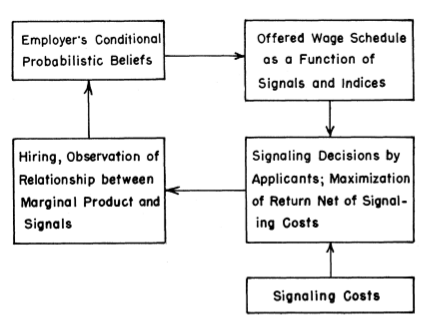
\includegraphics{fig-model-spence-informational-feedback.png}}
\end{figure}\end{frame}
%-------------------------------------------------------------------------------
%-------------------------------------------------------------------------------
\begin{frame}

We explore the following parameterized version.

\begin{align*}\begin{array}{l@{\qquad}l}
	h_L = 1   & h_H = 2 \\
	c_L = y   & c_H = \tfrac{1}{2}\,y \\
\end{array}\end{align*}

\end{frame}
%-------------------------------------------------------------------------------
%-------------------------------------------------------------------------------
\begin{frame}\begin{figure}[htp]\centering
\caption{Benefit of education}
\scalebox{0.35}{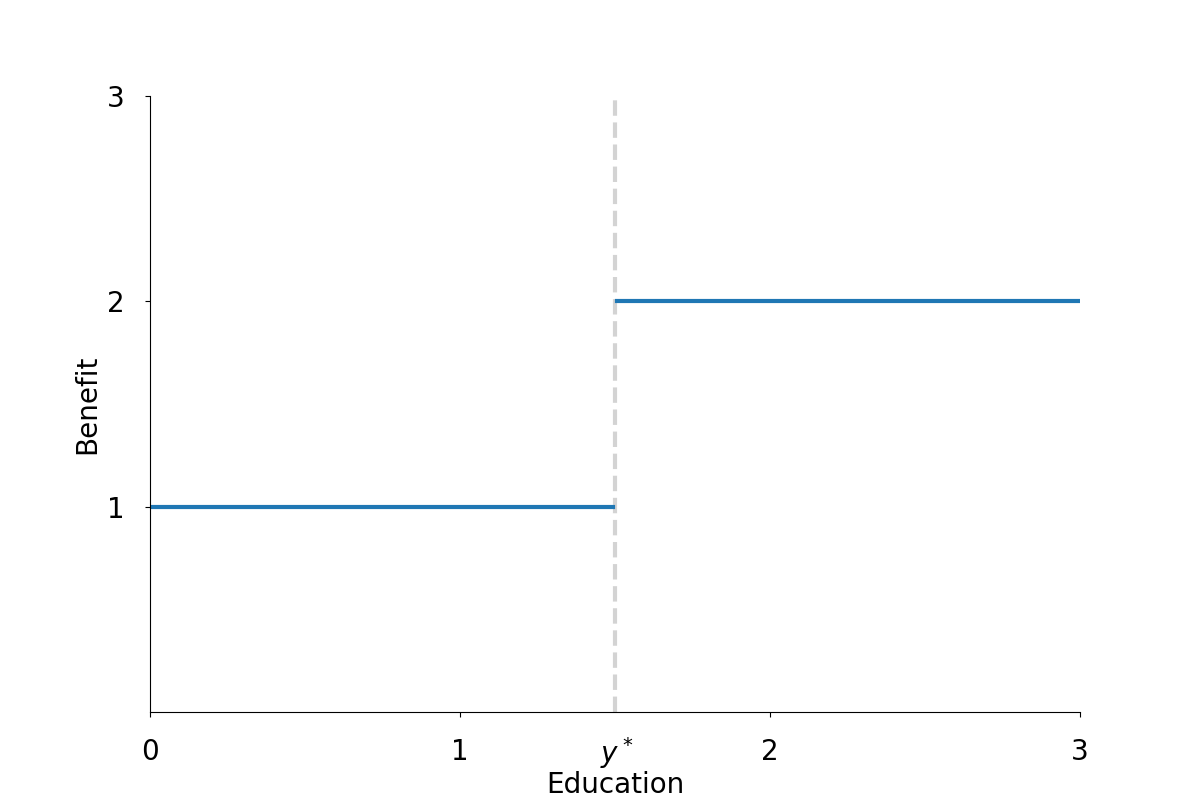
\includegraphics{fig-model-spence-benefit}}
\end{figure}\end{frame}
%-------------------------------------------------------------------------------
%-------------------------------------------------------------------------------
\begin{frame}\begin{figure}[htp]\centering
\caption{Cost of education}
\scalebox{0.35}{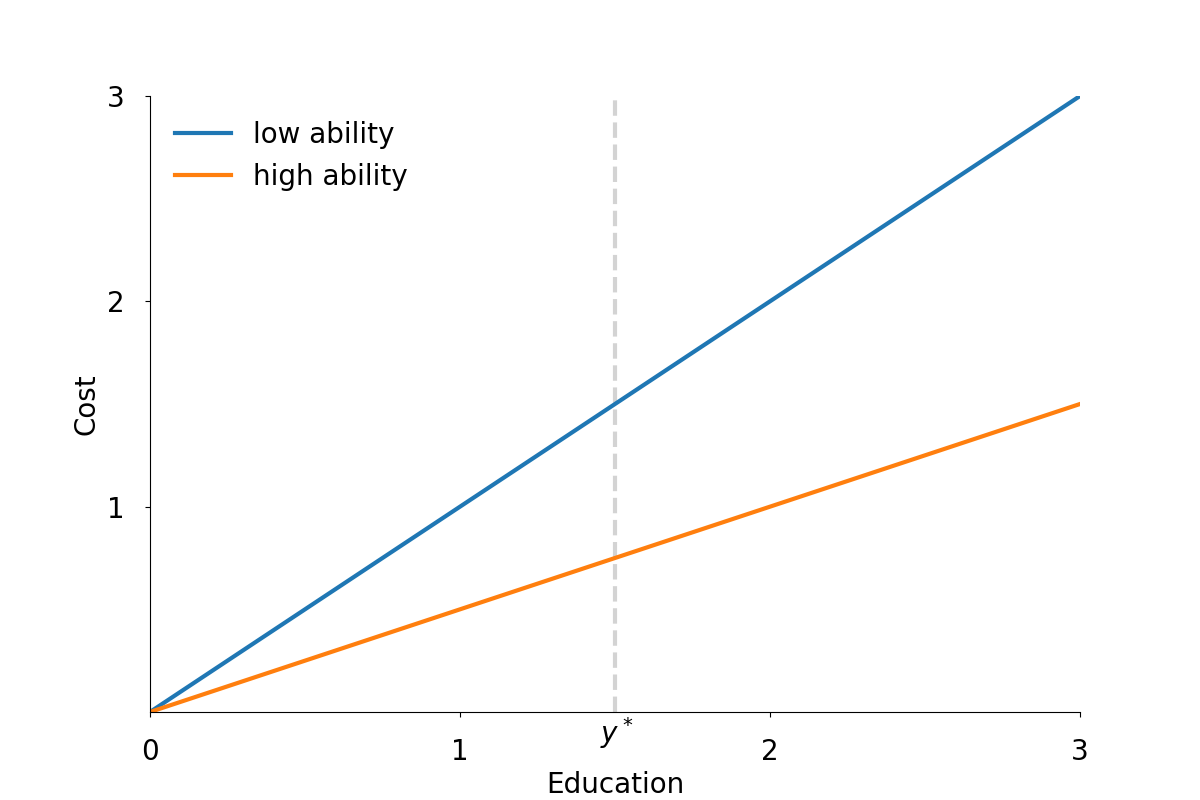
\includegraphics{fig-model-spence-cost}}
\end{figure}\end{frame}
%-------------------------------------------------------------------------------
%-------------------------------------------------------------------------------
\begin{frame}\begin{figure}[htp]\centering
\caption{Surplus of education I}
\scalebox{0.35}{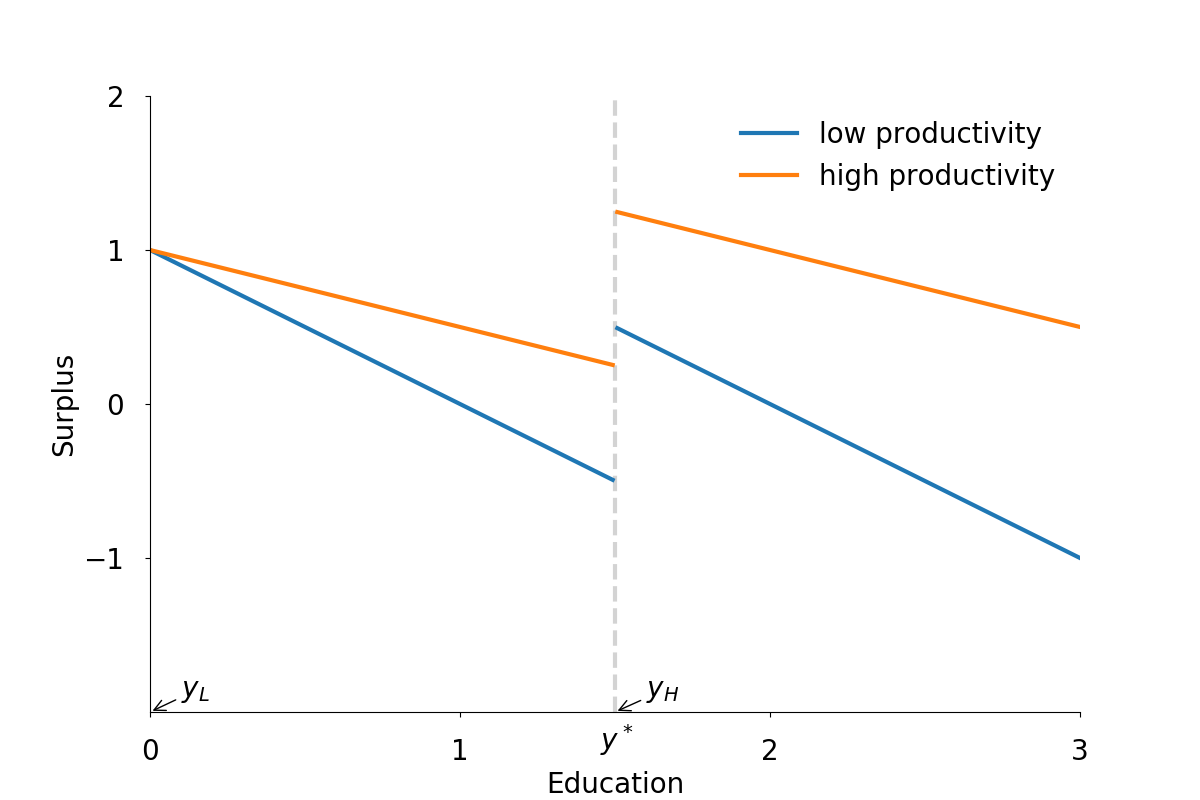
\includegraphics{fig-model-spence-surplus-base}}
\end{figure}\end{frame}
%-------------------------------------------------------------------------------
%-------------------------------------------------------------------------------
\begin{frame}
\begin{itemize}\setlength\itemsep{1em}
\item For $y^* = 1.5$ the employer's beliefs are confirmed. More generally, $L$ chooses $y_L = 0$ if $1 > 2 - y^*$ and $H$ acquires $y_H = y^*$ provided that $2 - 0.5\,y^* > 1$.
\item Beliefs are confirmed provided that the following holds:
	\begin{align*}
	1 < y^* < 2
	\end{align*}
\end{itemize}
\end{frame}
%-------------------------------------------------------------------------------
%-------------------------------------------------------------------------------
\begin{frame}\begin{figure}[htp]\centering
\caption{Surplus of education II}
\scalebox{0.35}{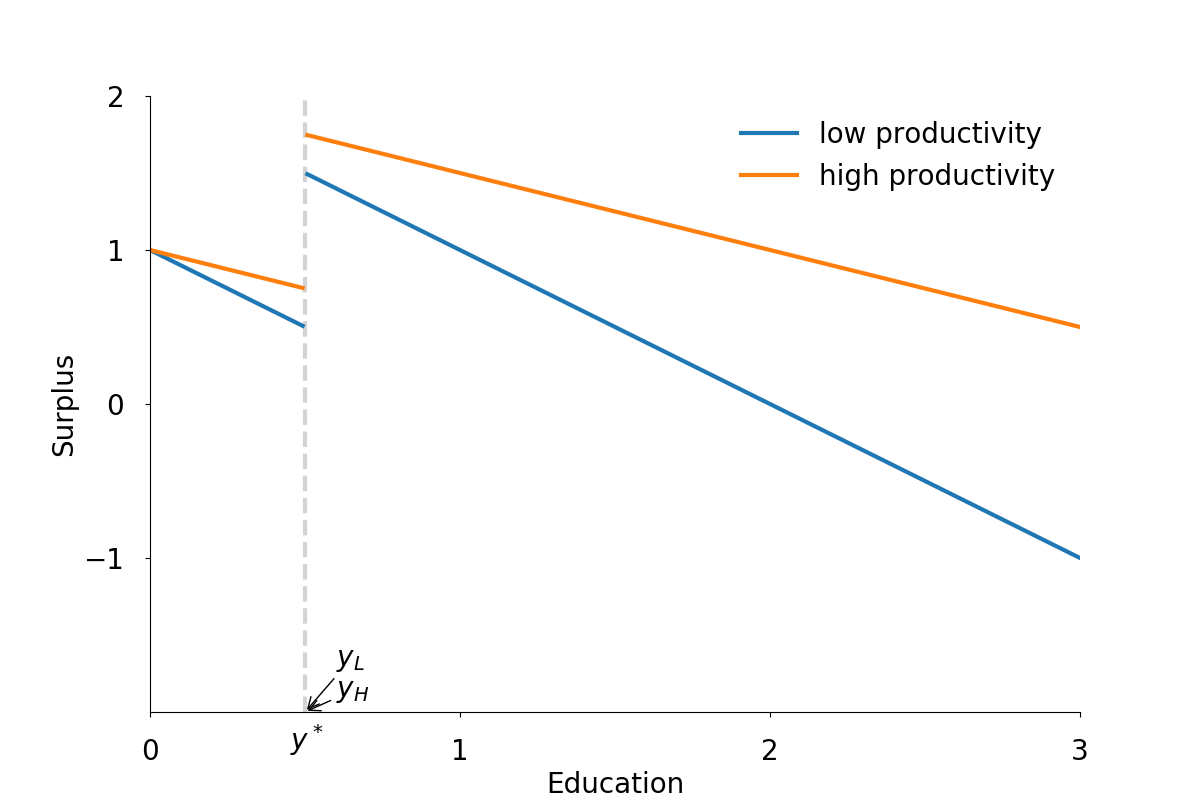
\includegraphics{fig-model-spence-surplus-low}}
\end{figure}\end{frame}
%-------------------------------------------------------------------------------
%-------------------------------------------------------------------------------
\begin{frame}
\begin{itemize}\setlength\itemsep{1em}
\item In the absence of signaling, both groups are paid the unconditional expected marginal product.
	\begin{align*}
	1\times q_L + (1 - q_L) \times 2
	\end{align*}
\end{itemize}
\end{frame}
